\documentclass[tikz,border=3mm]{standalone}
\usepackage{amsmath}
\usetikzlibrary{arrows.meta,calc,positioning}

\begin{document}
\pagecolor{white}
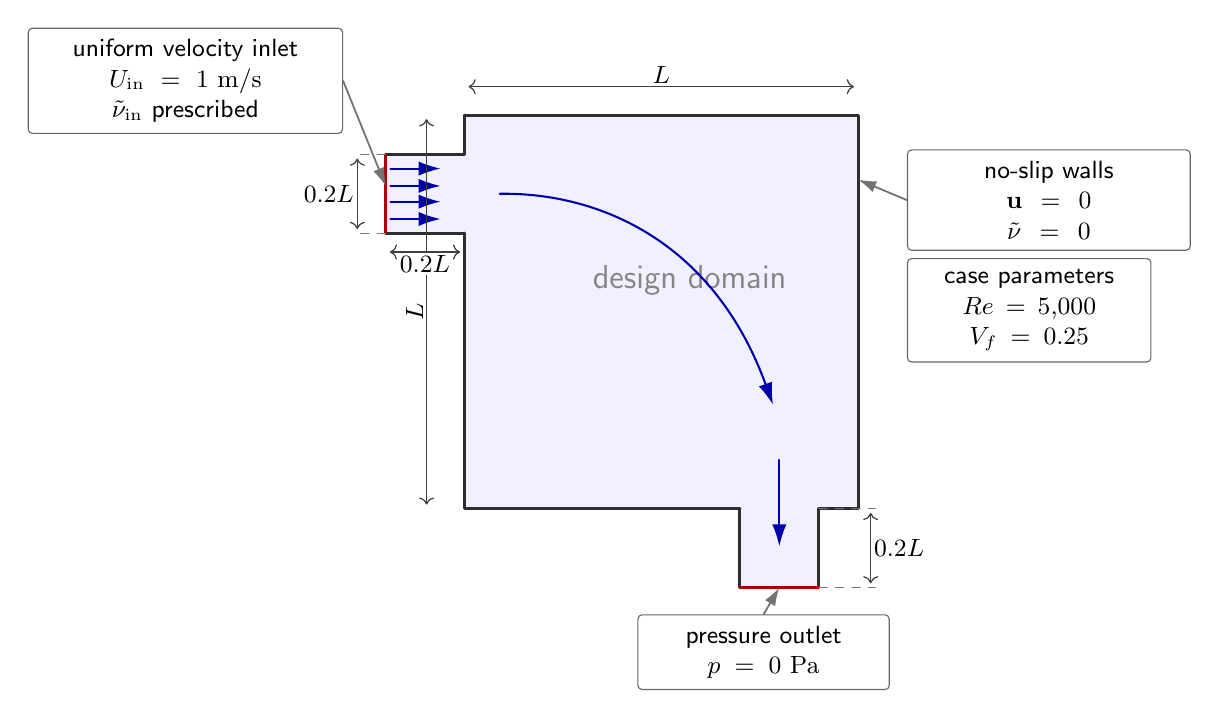
\begin{tikzpicture}[
  line cap=round,
  line join=round,
  font=\sffamily\small,
  flow/.style={-{Latex[length=2.8mm,width=1.8mm]}, line width=0.75pt, draw=blue!65!black},
  dim/.style={<->, line width=0.45pt, draw=black!75, shorten <=1.5pt, shorten >=1.5pt},
  bc/.style={draw=black!60, fill=white, rounded corners=1.5pt, inner xsep=7pt, inner ysep=4pt, align=center},
  wall/.style={draw=black!82, line width=1.1pt},
  boundary/.style={draw=red!70!black, line width=1.1pt},
  guide/.style={draw=black!55, dashed, line width=0.45pt},
  dimlabel/.style={fill=white, inner sep=1pt, font=\sffamily\small},
  designlabel/.style={font=\sffamily\large, text=black!48}
]

\def\L{5.0}
\def\lead{1.0}
\def\inletLow{3.5}
\def\inletHigh{4.5}
\def\inletMid{4.0}
\def\outletLowX{3.5}
\def\outletHighX{4.5}
\def\outletMidX{4.0}

% Design and non-design fluid regions.
\fill[blue!6] (0,0) rectangle (\L,\L);
\fill[blue!6] (-\lead,\inletLow) rectangle (0,\inletHigh);
\fill[blue!6] (\outletLowX,-\lead) rectangle (\outletHighX,0);
\node[designlabel] at (2.86,2.90) {design domain};

% No-slip walls.
\draw[wall] (0,\L) -- (\L,\L) -- (\L,0) -- (\outletHighX,0);
\draw[wall] (\outletLowX,0) -- (0,0) -- (0,\inletLow);
\draw[wall] (0,\inletHigh) -- (0,\L);
\draw[wall] (-\lead,\inletHigh) -- (0,\inletHigh);
\draw[wall] (-\lead,\inletLow) -- (0,\inletLow);
\draw[wall] (\outletLowX,-\lead) -- (\outletLowX,0);
\draw[wall] (\outletHighX,-\lead) -- (\outletHighX,0);

% Boundary sections.
\draw[boundary] (-\lead,\inletLow) -- (-\lead,\inletHigh);
\draw[boundary] (\outletLowX,-\lead) -- (\outletHighX,-\lead);

% Uniform inlet velocity and representative flow path.
\foreach \y in {3.68,3.90,4.10,4.32}{
  \draw[flow] (-0.94,\y) -- (-0.30,\y);
}
\draw[flow] (0.45,\inletMid) .. controls (1.75,4.02) and (3.18,3.36) .. (3.92,1.32);
\draw[flow] (4.00,0.62) -- (4.00,-0.48);

% Domain and port dimensions.
\draw[dim] (0,5.36) -- node[dimlabel, above] {$L$} (\L,5.36);
\draw[dim] (-0.48,0) -- node[dimlabel, midway, rotate=90, above] {$L$} (-0.48,\L);

\draw[guide] (-\lead,\inletHigh) -- (-1.42,\inletHigh);
\draw[guide] (-\lead,\inletLow) -- (-1.42,\inletLow);
\draw[dim] (-1.36,\inletLow) -- node[dimlabel, left] {$0.2L$} (-1.36,\inletHigh);
\draw[dim] (-\lead,\inletLow-0.24) -- node[dimlabel, below] {$0.2L$} (0,\inletLow-0.24);

\draw[guide] (\outletHighX,0) -- (5.22,0);
\draw[guide] (\outletHighX,-\lead) -- (5.22,-\lead);
\draw[dim] (5.16,-\lead) -- node[dimlabel, right] {$0.2L$} (5.16,0);

% Boundary-condition labels.
\node[bc, anchor=south east, text width=35mm] (inletLabel) at (-1.54,4.76)
  {uniform velocity inlet\\$U_{\mathrm{in}}=1~\mathrm{m/s}$\\$\tilde{\nu}_{\mathrm{in}}$ prescribed};
\draw[-{Latex[length=2.3mm,width=1.5mm]}, black!55, line width=0.65pt]
  (inletLabel.east) -- (-\lead,4.10);

\node[bc, anchor=north, text width=27mm] (outletLabel) at (3.80,-1.34)
  {pressure outlet\\$p=0~\mathrm{Pa}$};
\draw[-{Latex[length=2.3mm,width=1.5mm]}, black!55, line width=0.65pt]
  (outletLabel.north) -- (4.00,-\lead);

\node[bc, anchor=west, text width=31mm] (wallLabel) at (5.62,3.92)
  {no-slip walls\\$\mathbf{u}=0$\\$\tilde{\nu}=0$};
\draw[-{Latex[length=2.3mm,width=1.5mm]}, black!55, line width=0.65pt]
  (wallLabel.west) -- (5.00,4.18);

\node[bc, anchor=west, text width=26mm] at (5.62,2.52)
  {case parameters\\$Re=5{,}000$\\$V_f=0.25$};

\end{tikzpicture}
\end{document}
